\chapter{Introduzione}

La teoria che studieremo è una \textit{teoria geometrica}:

\textbf{I 5 postulati di Euclide:}
\begin{enumerate}
    \item Per due qualsiasi punti $A$ e $B$, esiste esattamente una retta che li attraversa.
    \item Una retta può essere prolungata indefinitamente in entrambe le direzioni.
    \item Dato un punto $O$ ed un raggio $R$, esiste esattamente un cerchio con centro in $O$ e raggio $R$.
    \item Tutti gli angoli retti sono congruenti.
    \item Data una retta $R$ ed un punto $P$ non appartenente a $R$, esiste esattamente una retta passante per $P$ che è parallela a $R$.
\end{enumerate}

Il quinto postulato è più complesso degli altri; nel corso del tempo, i matematici hanno provato più volte a dimostrare il quinto postulato basandosi sui restanti quattro. In seguito fu scoperto che il quinto è indipendente dagli altri.

\textbf{Conseguenze:}
\begin{enumerate}
    \item Non esiste alcuna retta parallela a $R$ passante per $P$ \\
    \quad $\rightarrow$ Geometrie ellittiche piane $[S^2]$
    \item Esistono due o più rette parallele a $R$ passanti per $P$ \\
    \quad $\rightarrow$ Geometrie iperboliche piane $[H^2]$
\end{enumerate}

\begin{figure}[H]
    \centering
    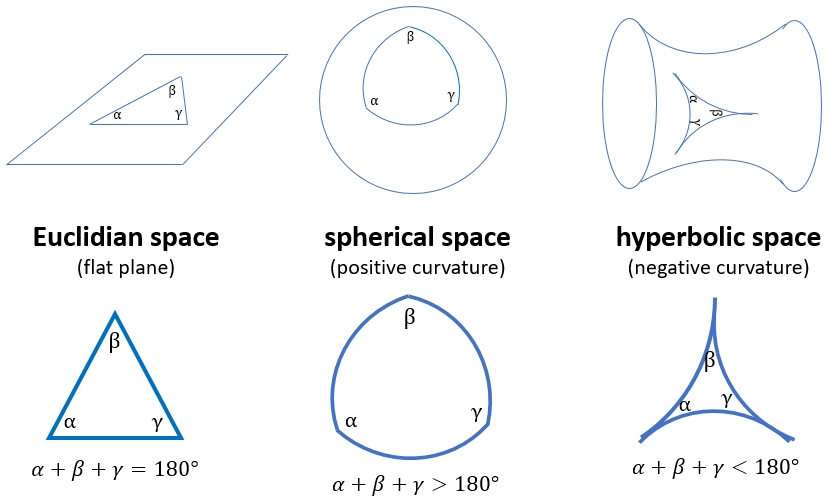
\includegraphics[width=0.5\textwidth]{assets/geometries.png}
    \caption{Geometrie ellittiche e iperboliche}
\end{figure}

\subsubsection{Geometria Ellittica}

La geometria ellittica piana è una forma di geometria non euclidea che rifiuta il quinto postulato di Euclide, il quale in geometria euclidea garantisce l'esistenza di una sola retta parallela passante per un dato punto. In geometria ellittica, non esistono rette parallele; invece, ogni coppia di rette si interseca eventualmente.

Un classico esempio è la geometria sferica, in cui le “rette” sono rappresentate da grandi cerchi su una sfera.

\begin{figure}[H]
    \centering
    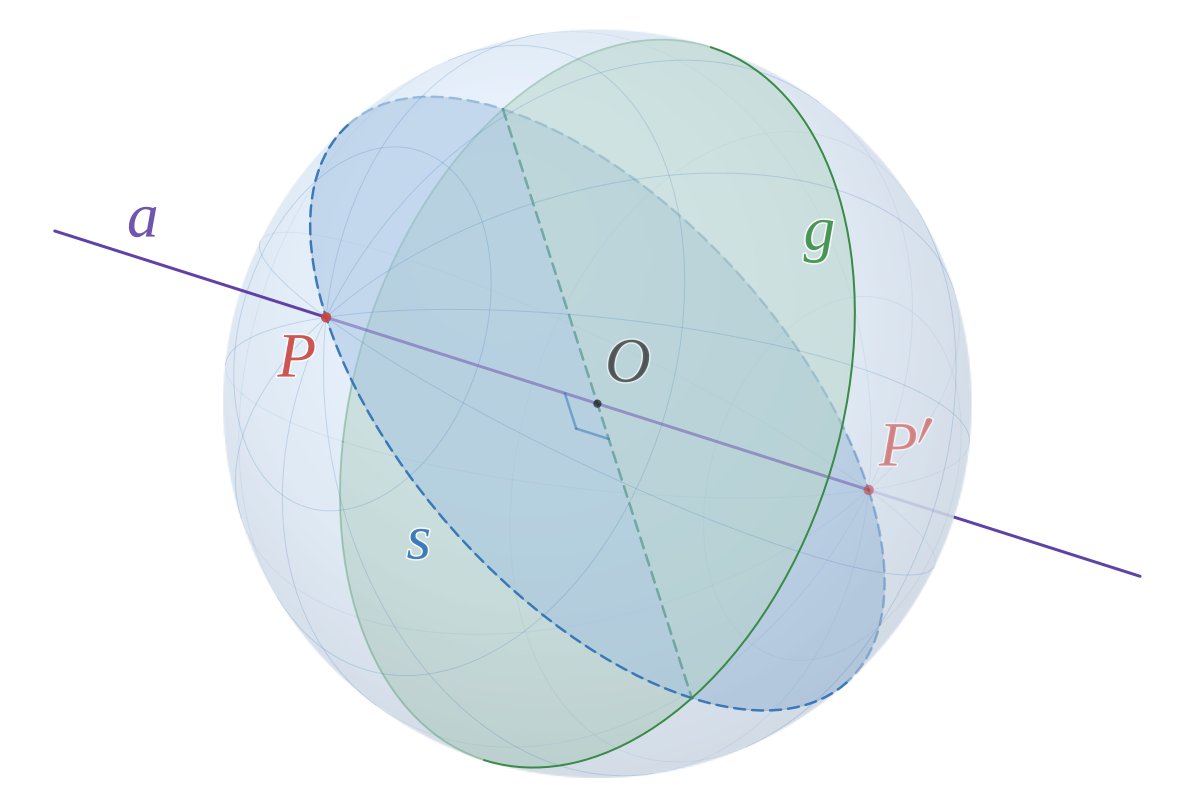
\includegraphics[width=0.5\textwidth]{assets/spherical_geometry.png}
    \caption{Geometria sferica}
\end{figure}

In questo contesto, i triangoli, noti come triangoli sferici, mostrano una proprietà intrigante: la somma dei loro angoli interni supera i 180° (un fenomeno noto come eccesso sferico), con l'eccesso proporzionale all'area del triangolo.

\begin{figure}[H]
    \centering
    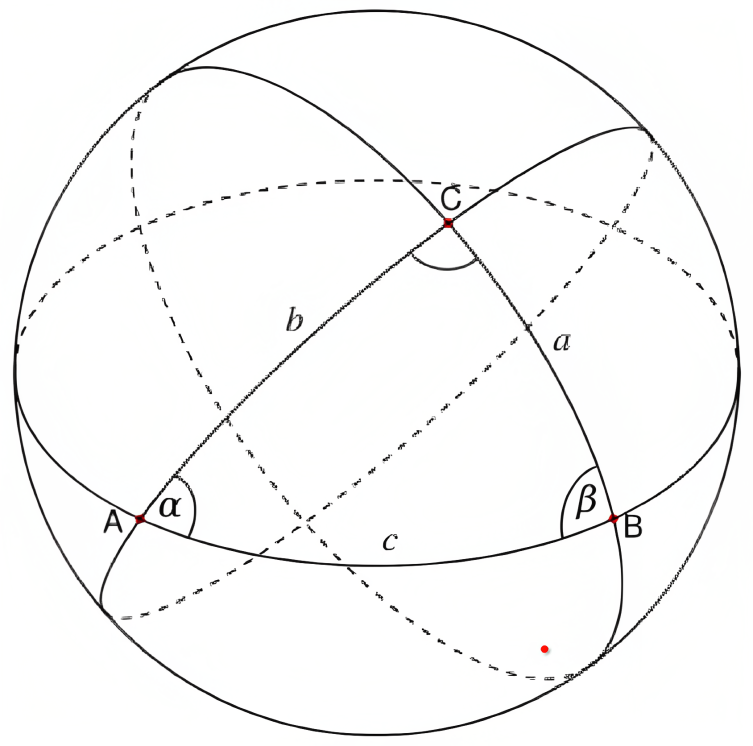
\includegraphics[width=0.5\textwidth]{assets/spherical_triangle.png}
    \caption{Triangolo sferico}
\end{figure}

\subsubsection{Geometria Iperbolica}

La geometria iperbolica piana è una forma di geometria non euclidea che rifiuta il quinto postulato di Euclide, il quale in geometria euclidea garantisce l'esistenza di una sola retta parallela passante per un dato punto. In geometria iperbolica, esistono molteplici rette parallele, e la somma degli angoli in un triangolo è sempre inferiore a 180°.

% \begin{figure}[H]
%     \centering
%     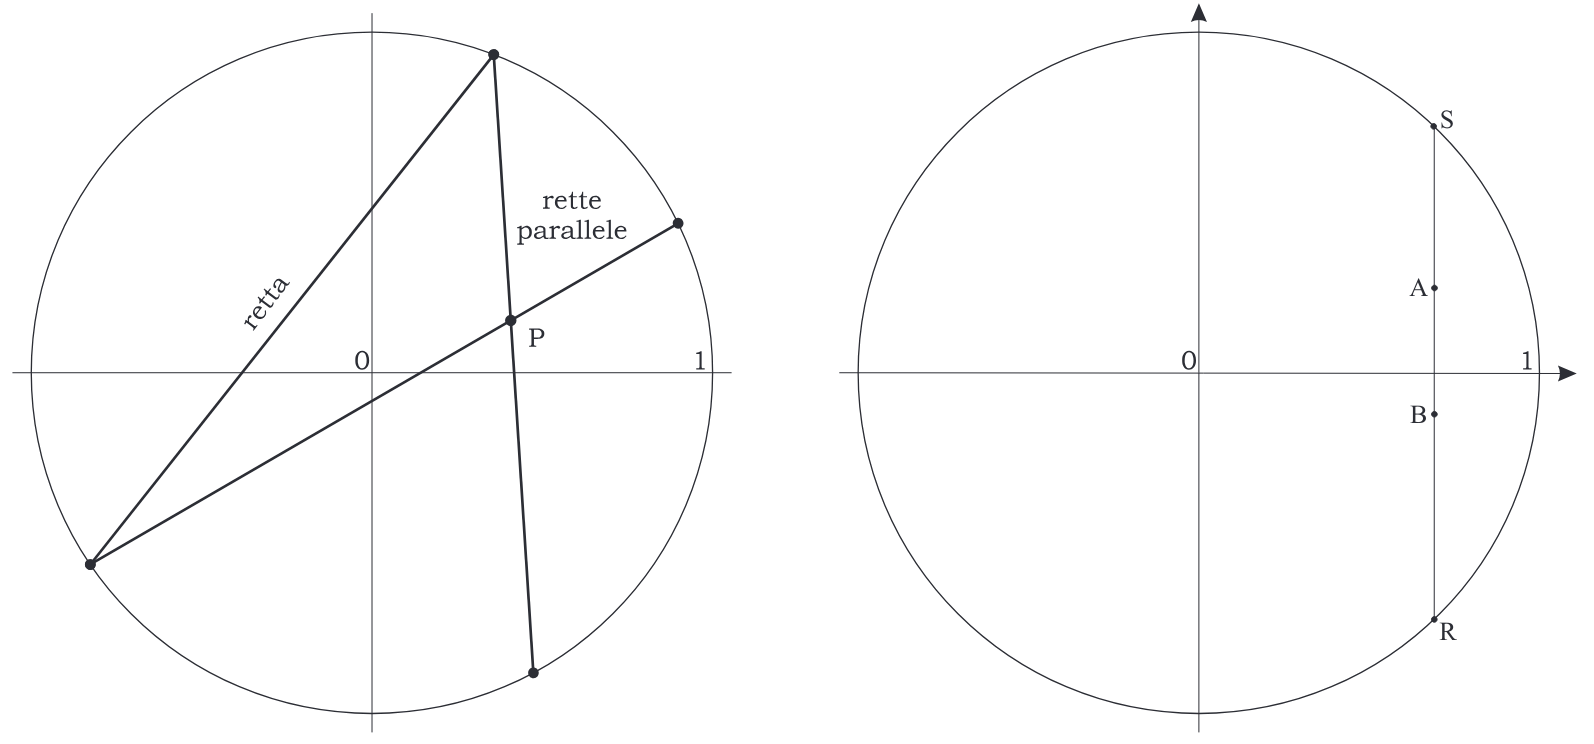
\includegraphics[width=0.5\textwidth]{assets/hyperbolic_geometry.png}
%     \caption{Geometria iperbolica}
% \end{figure}

In questo contesto, i triangoli, noti come triangoli iperbolici, mostrano una proprietà intrigante: la somma dei loro angoli interni è inferiore a 180°, con il difetto proporzionale all'area del triangolo.

\begin{figure}[H]
    \centering
    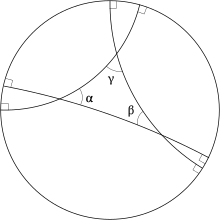
\includegraphics[width=0.5\textwidth]{assets/hyperbolic_triangle.png}
    \caption{Triangolo iperbolico}
\end{figure}

\subsubsection{Curva piana}

\textbf{Ascissa curvilinea}

\dots

\newpage

L'altra volta abbiamo visto come poter usare le coordinate curvilinee per descrivere tre geometrie.
Abbiamo visto poi come 

Ora iniziamo a ragionare con le superfici.

Supponiamo di avere un dominio $D \in \mathbb{R}^2$ e di voler mappare $D$ in un sistema a 3 dimensioni:

$$
\bar{x}(u,v) = (x_1, x_2, x_3) = (x_1(u,v), x_2(u,v), x_3(u,v))
$$

Calcoliamo il gradiente di $\bar{x}$ rispetto a $u$ e $v$:

$$
\begin{cases}
\bar x_u = \frac{\partial \bar x}{\partial u} = \left( \frac{\partial x_1}{\partial u}, \frac{\partial x_2}{\partial u}, \frac{\partial x_3}{\partial u} \right)
\\
\bar x_v =\frac{\partial \bar x}{\partial v} = \left( \frac{\partial x_1}{\partial v}, \frac{\partial x_2}{\partial v}, \frac{\partial x_3}{\partial v} \right)
\end{cases}
$$

Il versore normale alla superficie è dato da:

$$
\hat {n} = \dfrac{\bar x_u \times \bar x_v}{|\bar x_u \times \bar x_v|}
$$

Si dice che la superficie $M$ è regolare (smooth) se il versore normale è ben definito e non nullo, ovvero $\bar x_u$ e $\bar x_v$ non sono paralleli:

$$
\bar x_u \times \bar x_v \neq 0
$$

\subsubsection{Superficie di una sfera di raggio R}

Consideriamo una sfera di raggio $R$ centrata nell'origine. La superficie della sfera è data da:

$$
\bar x(u,v) = (R \cos u \cos v, R \sin u \cos v, R \sin v)
$$
dove $u \in [-\pi, \pi]$, $v \in [-\pi/2, \pi/2]$

\vspace{0.5em}

Calcoliamo il gradiente di $\bar x$ rispetto a $u$ e $v$:

$$
\begin{cases}
\bar x_u = \frac{\partial \bar x}{\partial u} (-R \sin u \cos v, R \cos u \cos v, 0)
\\
\bar x_v = \frac{\partial \bar x}{\partial v} = (-R \cos u \sin v, -R \sin u \sin v, R \cos v)
\end{cases}
$$

Andiamo ad analizzare il punto $(u,v) = (0,0)$:
$$
\begin{cases}
\bar x_u = (0, R, 0)
\\
\bar x_v = (0, 0, R)
\end{cases}
$$

Questi due vettori individuano la superficie tangente alla sfera nel punto $(0,0)$.

Il versore normale alla superficie è dato da:

$$
\hat {n} = \dfrac{\bar x_u \times \bar x_v}{|\bar x_u \times \bar x_v|} = \dfrac{(-R^2, 0, 0)}{R^2} = (-1, 0, 0)
$$

\newpage

\section{Prima Forma Fondamentale}

In geometria differenziale, la \emph{Prima Forma Fondamentale} fornisce la metrica intrinseca di una superficie. Essa permette di calcolare lunghezze, angoli e aree sulla superficie, misurando come essa si deforma nelle diverse direzioni. Consideriamo una superficie liscia parametrizzata da $\bar{x}(u,v)$, dove $u$ e $v$ sono le coordinate locali. I vettori tangenti alla superficie sono definiti da:

$$
\bar{x}_u = \frac{\partial \bar{x}}{\partial u}, \quad \bar{x}_v = \frac{\partial \bar{x}}{\partial v}.
$$

I coefficienti della prima forma sono:

$$
E = \bar{x}_u \cdot \bar{x}_u,\quad F = \bar{x}_u \cdot \bar{x}_v,\quad G = \bar{x}_v \cdot \bar{x}_v.
$$

Un elemento di spostamento infinitesimale sulla superficie si esprime come combinazione lineare dei vettori tangenti. Espandendo il quadrato dello spostamento, otteniamo:

$$
u^2\underbrace{\left(\bar{x}_u \cdot \bar{x}_u\right)}_E + 2uv\underbrace{\left(\bar{x}_u \cdot \bar{x}_v\right)}_F + v^2\underbrace{\left(\bar{x}_v \cdot \bar{x}_v\right)}_G,
$$
da cui il quadrato dell'elemento di lunghezza diventa

$$
ds^2 = E\,du^2 + 2F\,du\,dv + G\,dv^2.
$$

Se una curva sulla superficie è parametrizzata da un parametro $t$, con $u = u(t)$ e $v = v(t)$, allora derivando si ottiene:
$$
\frac{ds^2}{dt^2} = E\, u^2 + 2F\,uv + G\,v^2.
$$

Pertanto, la lunghezza $L$ della curva, per $t$ compreso tra $a$ e $b$, si calcola come:

$$
L = \int_a^b \frac{ds}{dt}\, dt = \int_a^b \sqrt{E\, u^2 + 2F\,uv + G\,v^2}\, dt.
$$

In alternativa, esprimendo direttamente la lunghezza lungo la curva $\bar{r}$ sulla superficie, si ha:

$$
L = \int_{\bar{r}} ds = \int_{\bar{r}} \sqrt{E\,du^2 + 2F\,du\,dv + G\,dv^2}.
$$

Questa formulazione riassume le proprietà geometriche intrinseche della superficie, permettendo di misurare le distanze in maniera indipendente dallo spazio ambiante.


\subsection{Sfera in coordinate sferiche}

Consideriamo una sfera di raggio $R$ centrata nell'origine.La superficie della sfera è data da:

\small
$$
\bar x(u,v) = (R \cos u \cos v, R \sin u \cos v, R \sin v)
\quad \xrightarrow{\text{derive}} \quad
\begin{cases}
    \bar x_u = (-R \sin u \cos v, R \cos u \cos v, 0)
    \\
    \bar x_v = (-R \cos u \sin v, -R \sin u \sin v, R \cos v)
\end{cases}
$$
\normalsize

dove $u \in [-\pi, \pi]$, $v \in [-\pi/2, \pi/2]$

Calcoliamo i coefficienti della prima forma fondamentale:

$$
\begin{cases}
E = \bar{x}_u \cdot \bar{x}_u = R^2 \sin^2 v \cos^2 u + R^2 \sin^2 v \sin^2 u = R^2 \sin^2 v
\\
F = \bar{x}_u \cdot \bar{x}_v = R^2 \sin v \cos v \cos u \cos u + R^2 \sin v \cos v \sin u \sin u = 0
\\
G = \bar{x}_v \cdot \bar{x}_v = R^2 \cos^2 v
\end{cases}
$$

Quindi, la prima forma fondamentale è:

$$
ds^2 = R^2 \sin^2 v\, du^2 + R^2 \cos^2 v\, dv^2
$$

\subsection{Forma metrica}

La forma metrica è una generalizzazione della prima forma fondamentale, che permette di calcolare la lunghezza di curve e la misura di angoli su una superficie. La forma metrica è definita come:

$$
g = E\,du^2 + 2F\,du\,dv + G\,dv^2
$$

dove $E$, $F$ e $G$ sono i coefficienti della prima forma fondamentale. La forma metrica è una forma bilineare simmetrica, che può essere rappresentata da una matrice:

$$
\begin{pmatrix}
    a & b \\
\end{pmatrix}
\underbrace{
\begin{pmatrix}
E & F \\
F & G
\end{pmatrix}
}_{\small \text{Forma metrica}}
\begin{pmatrix}
    c \\
    d
\end{pmatrix}
$$

\subsection{Identità di Lagrange}

L'identità di Lagrange è una relazione che lega la forma metrica e la prima forma fondamentale di una superficie.

$$
\bar x_u \times \bar x_v \neq 0 \quad \Rightarrow \quad \hat N = \dfrac{\bar x_u \times \bar x_v}{|\bar x_u \times \bar x_v|}
$$

L'identità di Lagrange afferma che:

$$
|\bar x_u \times \bar x_v|^2 =
\det
\begin{pmatrix}
    E & F \\
    F & G
\end{pmatrix}
$$

\subsubsection{Dimostrazione}

Iniziamo considerando il prodotto vettoriale tra $\bar x_u$ e $\bar x_v$:

$$
\bar x_u \times \bar x_v = |\bar x_u| |\bar x_v| cos \theta
$$

dove $\theta$ è l'angolo tra $\bar x_u$ e $\bar x_v$. Elevando al quadrato, otteniamo:

$$
|\bar x_u \times \bar x_v|^2 = (|\bar x_u|^2 |\bar x_v|^2 \sin^2 \theta) = |\bar x_u|^2 |\bar x_v|^2 (1 - \cos^2 \theta) = \underbrace{|\bar x_u|^2}_E \cdot \underbrace{|\bar x_v|^2}_G - \underbrace{(\bar x_u \cdot \bar x_v)^2}_{F^2}
$$

Ricordando che $|\bar x_u \times \bar x_v|^2 = \det \begin{pmatrix} E & F \\ F & G \end{pmatrix}$, otteniamo l'identità di Lagrange:

$$
\det \begin{pmatrix} E & F \\ F & G \end{pmatrix} = EG - F^2
$$

\dots

\newpage

$$
g_{ij} = \begin{pmatrix}
    g_{11} & g_{12} \\
    g_{21} & g_{22}
\end{pmatrix}
$$

$$
g_{i,j} = \bar x_i \cdot \bar x_j
$$

$$
\vec v = \sum_i v^i \bar x_i
$$
$$
\vec w = \sum_j w^j \bar x_j = 
$$

forma matriciale tensore metrico

$$
ds^2 = g_{ij} du^i du^j
$$
